% Semantic-minimal TikZ template (default profile; see references/tikz-semantic-minimal.md).
% English figure: pdflatex + newtx. Chinese figure: replace the two font lines with
%   % !TEX program = xelatex   (must be the first line)
%   \usepackage{fontspec}\usepackage{xeCJK}
%   \setmainfont{Times New Roman}\setCJKmainfont{Songti SC}[BoldFont=Heiti SC]
\documentclass[tikz,border=6pt]{standalone}
\usepackage{newtxtext,newtxmath}
\usetikzlibrary{positioning,arrows.meta,calc,backgrounds}

% structure grays
\definecolor{ink}{RGB}{64,64,64}
\definecolor{muted}{RGB}{120,120,120}
\definecolor{optF}{RGB}{242,242,242}
\definecolor{bandA}{RGB}{247,247,247}\definecolor{bandB}{RGB}{238,238,238}
% semantic pairs (F fill / D draw); use at most three, each with one declared meaning
\definecolor{sAF}{RGB}{226,236,247}\definecolor{sAD}{RGB}{38,84,140}   % A blue
\definecolor{sBF}{RGB}{251,229,211}\definecolor{sBD}{RGB}{176,84,26}   % B orange (key)
\definecolor{sCF}{RGB}{224,240,226}\definecolor{sCD}{RGB}{46,110,62}   % C green

\begin{document}
% Coordinate ledger (replace before drawing; ASCII only):
% target width = ... mm
% columns x = 2.0, 5.6, 9.2      lanes y = 3.6, 1.2
% node width = 28mm, height = 13mm, gap = 0.8cm
% feedback routing lane: y = -0.3
% semantic map: A = ..., B = ..., C = ...   (delete unused pairs)
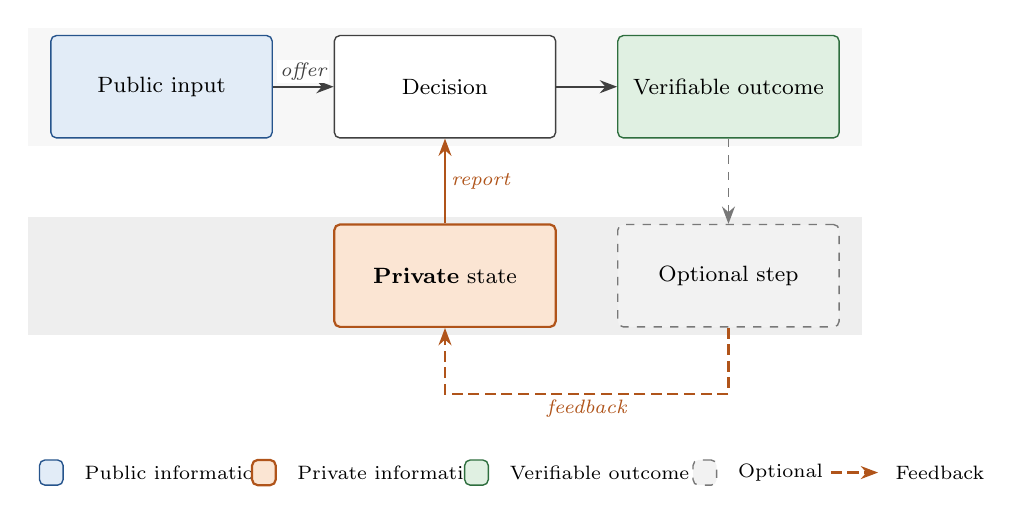
\begin{tikzpicture}[
  font=\footnotesize,
  >={Stealth[length=2.2mm]},
  box/.style={draw=ink, fill=white, rounded corners=2pt, align=center,
              minimum height=13mm, text width=#1, inner sep=3pt, line width=0.5pt},
  box/.default=26mm,
  semA/.style={box=#1, draw=sAD, fill=sAF},   semA/.default=26mm,
  semB/.style={box=#1, draw=sBD, fill=sBF, line width=0.8pt}, semB/.default=26mm,
  semC/.style={box=#1, draw=sCD, fill=sCF},   semC/.default=26mm,
  opt/.style={box=#1, draw=muted, fill=optF, dashed}, opt/.default=26mm,
  flow/.style={->, line width=0.6pt, ink},
  back/.style={->, line width=0.8pt, sBD, dash pattern=on 4pt off 2pt},
  lbl/.style={font=\scriptsize\itshape, fill=white, inner sep=1pt},
]

% lanes (optional, light gray only)
\fill[bandA] (0.3,2.85) rectangle (10.9,4.35);
\fill[bandB] (0.3,0.45) rectangle (10.9,1.95);

% nodes: replace with the method- and benchmark-driven layout
\node[semA] (a) at (2.0,3.6) {Public input};
\node[box]  (b) at (5.6,3.6) {Decision};
\node[semB] (c) at (5.6,1.2) {\textbf{Private} state};
\node[semC] (d) at (9.2,3.6) {Verifiable outcome};
\node[opt]  (e) at (9.2,1.2) {Optional step};

\draw[flow] (a) -- node[lbl, above=1pt]{offer} (b);
\draw[flow, sBD] (c.north) -- node[lbl, right=1pt, text=sBD]{report} (b.south);
\draw[flow] (b) -- (d);
\draw[flow, dashed, muted] (d.south) -- (e.north);
\draw[back] (e.south) -- (9.2,-0.3) -- (5.6,-0.3)
  node[lbl, midway, below=1pt, text=sBD]{feedback} -- (c.south);

% legend: list only encodings that actually appear
\begin{scope}[shift={(0.6,-1.3)}]
  \node[semA=3mm, minimum height=3.2mm, inner sep=0pt] at (0,0) {};
  \node[anchor=west, font=\scriptsize] at (0.3,0) {Public information};
  \node[semB=3mm, minimum height=3.2mm, inner sep=0pt] at (2.7,0) {};
  \node[anchor=west, font=\scriptsize] at (3.0,0) {Private information};
  \node[semC=3mm, minimum height=3.2mm, inner sep=0pt] at (5.4,0) {};
  \node[anchor=west, font=\scriptsize] at (5.7,0) {Verifiable outcome};
  \node[opt=3mm, minimum height=3.2mm, inner sep=0pt] at (8.3,0) {};
  \node[anchor=west, font=\scriptsize] at (8.6,0) {Optional};
  \draw[back] (9.9,0) -- (10.5,0);
  \node[anchor=west, font=\scriptsize] at (10.6,0) {Feedback};
\end{scope}
\end{tikzpicture}
\end{document}
